\singlespacing
\chapter{Le Grand Collisionneur de Hadrons (LHC) et le détecteur
  ATLAS}
\label{sec:lhc_atlas}
\doublespacing{}

\section{Le LHC}
\label{sec:lhc_atlas:lhc}

% intro
Le Grand Collisioneur de Hadron~\cite{evans_lhc_2008}, noté
LHC~\footnote{De l'anglais \emph{Large Hadron Collider}}, est un
accélérateur de particules situé au CERN sur la fontière franco-suisse
près de Genève le long d'un tunnel circulaire de 27 km de
circonférence.  Ce tunnel a été creusé dans les années 80 pour
aceuillir le collisioneur électron-positron LEP qui a été en opération
jusqu'en 2000 pour ensuite céder sa place au LHC.

Le LHC est un accélérateur de hadron utilisé principalement pour
collisioneur deux faisceaux de protons et aussi, dans une moindre
mesure, pour des collisions plomb-plomb ou plomb-proton. Il opère
présentement à une énergie de 6.5 TeV par faisceau par nucléon, en
faisant l'accélérateur de particules le plus puissant à ce
jour~\cite{olive_parameters_2014}.

% détecteurs
Il y a au total sept détecteurs installé le long du LHC:
\def\labelitemi{$\bullet$}
\begin{itemize}
\item \textbf{ATLAS}~\cite{collaboration_atlas_2008}: Détecteur
  d'usage général, est décrit en détail dans la
  section~\ref{sec:lhc_atlas:atlas}.
\item \textbf{CMS}~\cite{collaboration_cms_2008}: Détecteur d'usage
  général. Expérience soeur d'ATLAS.
\item \textbf{LHCb}~\cite{nakada_lhcb_2000}: Détecteur optimisé pour
  les études sur la physique des mésons B.
\item \textbf{ALICE}~\cite{collaboration_alice_2008}: Détecteur dédié
  aux collions d'ions lourds (plomb-plomb ou proton-plomb).
\item \textbf{LHCf}~\cite{collaboration_lhcf_2008}: Installé
  directement sur la ligne de faisceau près d'ATLAS pour étudier le
  spectre énergétrique des particules produites quasi-parallèment au
  faisceau lors de collisions dans ATLAS.
\item \textbf{TOTEM}~\cite{collaboration_totem_2008}: Installé près de
  CMS, dédié aux mesures de sections efficaces totales proton-proton
  et à l'étude de la structure du proton en mesurant les particules
  produites à petits angles lors de collisions dans CMS.
\item \textbf{MoEDAL}~\cite{Pinfold:1181486}: Installé près de LHCb,
  utilisé pour chercher le monopole magnétique. \\
\end{itemize}

Les expériences ATLAS et CMS visent une haute luminosité
$L = 10^{34} cm^2 s^1$, ce qui représente 40 millions de collisons
entre paquets de protons à toutes les
secondes~\cite{collaboration_atlas_2008}. La luminosité dépendant du
nombre de particules dans chaque paquet et linéairement du nombre de
paquets, il est crucial d'obtenir des faisceau de très hautes
intensités, ce qui exclu l'utilisation de faisceaux d'anti-protons
qui sont difficiles à produire. Cela complique la conception de la
ligne de faisceau puisqu'il doit y avoir deux champs éléctromagnétique
dans des directions opposées pour accélérer les deux faisceaux de
protons. Il y a donc, en réalité, deux lignes de faisceau, comme
montré dans la figure~\ref{fig:dipole}~\cite{evans_lhc_2008}.

\begin{figure}
  \centering
  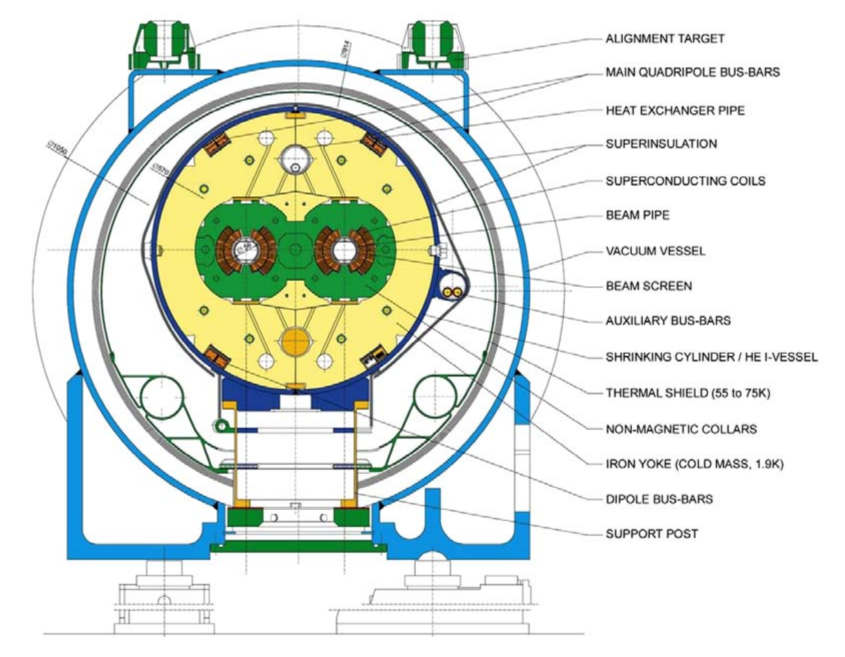
\includegraphics[width=.5\textwidth]{dipole.pdf}
  \caption{Coupe d'un aimant dipole du LHC, où on voit les deux lignes
    de faisceau où les protons voyagent en sexns opposés. Figure tirée
    de la référence~\cite{evans_lhc_2008}}
\label{fig:dipole}
\end{figure}

% chaine d'accélération
Le LHC est conçu pour accélérer des protons d'une énergie initiale de
450 GeV à une énergie finale de 6.5 TeV. Puisque les protons doivent
avoir une énergie considérable dès leur injection dans le LHC, il doit
nécessairement y avoir un accélérateur en amont. En réalité, ce sont
quatres accélérateurs différents, déjà présents sur le site du CERN
avant la construction du LHC, qui servent de ligne d'injection (voir
figure~\ref{fig:lhc_injection}. Au tout début se trouve le LINAC II,
un accélérateur linéaire. Le faisceau initial est ensuite transféré
succesivement dans le \emph{proton-synchrotron booster},
\emph{proton-synchrotron} et le \emph{super-proton-synchrotron}, pour
finalement être transféré au LHC~\cite{evans_lhc_2008}.

\begin{figure}
  \centering
  \includegraphics{lhc_injection.pdf}
  \caption{Ligne d'injection du LHC. Figure tiré de la
    référene~\cite{Lefevre:1165534}}
  \label{fig:lhc_injection}
\end{figure}



%% atlas
%% cms
%% lhcb
%% alice
%% LHCf
%% totem
%% moedal

\section{Le détecteur ATLAS}
\label{sec:lhc_atlas:atlas}

\subsection{Le détecteur interne}
\label{sec:lhc_atlas:atlas:indet}

\subsection{Les calorimètres}
\label{sec:lhc_atlas:atlas:calo}

\subsection{Le spectromètre à muon}
\label{sec:lhc_atlas:atlas:mu}

\subsection{Aquisition des données}
\label{sec:lhc_atlas:atlas:daq}

%%% Local Variables:
%%% mode: latex
%%% TeX-master: "memoire" 
%%% End:
